%++++++++++++++++++++++++++++++++++++++++
% Don't modify this section unless you know what you're doing!
\documentclass[letterpaper,12pt]{article}
\usepackage{tabularx} % extra features for tabular environment
\usepackage{amssymb, amsfonts,amssymb,amscd,amsbsy}
\usepackage{amsmath, amsthm}  % improve math presentation
\usepackage{graphicx} % takes care of graphic including machinery
\usepackage[margin=1in,letterpaper]{geometry} % decreases margins
\usepackage{cite} % takes care of citations
\usepackage[final]{hyperref} % adds hyper links inside the generated pdf file
\usepackage{float}
\usepackage{booktabs}
\usepackage{graphicx}
\usepackage{tikz}
\usepackage{fancyhdr}
\usepackage{lastpage}
\usepackage{lipsum}

\DeclareMathOperator*{\argmin}{arg\,min} % thin space, limits underneath in displays
\DeclareMathOperator*{\argmax}{arg\,max} % thin space, limits underneath in displays

\renewcommand*\contentsname{Table of Contents}
\setlength{\headheight}{15pt}
\setlength{\footskip}{45pt}

\hypersetup{
	colorlinks=true,       % false: boxed links; true: colored links
	linkcolor=blue,        % color of internal links
	citecolor=blue,        % color of links to bibliography
	filecolor=magenta,     % color of file links
	urlcolor=blue         
}
%++++++++++++++++++++++++++++++++++++++++

\title{\textbf{Main Title or Report Id} \\ Title} % Example TH: Thesis, Year, Progress Number, Report Number R..: TH202201R01
\def\shorttitle{ Short Title } % For header of the document
\def\labwebpage{\url{https://kontrol.itu.edu.tr/en/research/laboratories/robotics-laboratory} \\ \url{https://github.com/ITUROBLAB}} % ITUROBLAB webpage link

\author{Name SURNAME, Second AUTHOR, Third AUTHOR}
\date{\today} % or if you want to add a specific date use \date{20 Ekim 2017} \today

\begin{document}

\makeatletter
    \begin{titlepage}
        \begin{center}
            \vspace*{0.7cm}
            \rule{14cm}{3pt}\\
            {\LARGE \@title }\\[7ex] 
            
\includegraphics[width=0.3\linewidth]{figs/ITUROBLAB.png}\\[-2ex]
            {\scriptsize \labwebpage}\\
            \rule{2cm}{0.5pt}\rule[0.5mm]{2cm}{2pt}\rule[-0.5mm]{2cm}{2pt}\rule[0.5mm]{2cm}{2pt}\rule{2cm}{0.5pt}\\[4ex]
            {\large \@author}\\[1ex] 
            {\normalsize \@date}\\ [1ex]
            \rule{14cm}{0.5pt}
            {\begin{abstract}
            %% Add abstract of your report %%
            In this report, ... Give abstract in a single paragraph (summary of your report including what you did, why you did, what you obtained, the repository link where the details can be found, and superiority of your achievement, if any).\lipsum[1]
            %%%%%%%%%%%%%%%%%%%%%%%%%%%%%%%
            \end{abstract}}
        \end{center}
        \tikz [remember picture, overlay] %
        \node [shift={(-2.4cm,0.5cm)}] at (current page.south east) %
        [anchor=south east] %
        {
\includegraphics[width=1cm]{figs/ituLogo.png}};
    \end{titlepage}
\makeatother
%\thispagestyle{empty}

\pagestyle{fancy}
\fancyhf{}
\rhead{\shorttitle}
%\lhead{Guides and tutorials}
\lfoot{Page \thepage \hspace{1pt} of \pageref{LastPage}}
\rfoot{
\includegraphics[width=1cm]{figs/ituLogo.png}}

\tableofcontents

%% If you write a long report, add list of figures and tables and start reporting on new page
%\listoffigures
%\listoftables
%\newpage

\section{Problem Definition}

Paper reference (citation) Du et al. \cite{du2010affine} ... Adding equation reference \eqref{eq:integralli} ... In line equation mode $\lim\limits_{x \rightarrow 3}$ to give equation in a sentence.

\begin{equation}
\label{eq:integralli} % the label is used to reference the equation
\dot{x}(t) = \int\limits_{0}^{\tau} x(t) dt
\end{equation}

\noindent
where $\dot{x}(t)$ is velocity of the mass and ...

\subsection{Adding sub-section}

Multi line equations example:

\begin{align} % & for aligning
x_1&=3 + y^2 \\
&= a^2  \nonumber \\  % do not add number for this line
&= b^2
\end{align}

\subsubsection{Adding sub-sub-section}

\lipsum[3]

\section{Second Section}

The objective function in \eqref{eq:objective} can be maximized .... If we define $\vec{\bar{p}}_i\triangleq \left[\vec{p}_i^T, 1 \right]^T$ and ..., the compact form of the equation is achieved as 

\begin{equation}
\label{eq:objective}
\sum_{i=1}^{\mathit{N_p}}\exp \left( -\dfrac{\lVert\mathbb{A}\vec{\bar{p}}_i-\vec{\bar{m}}_{c_{k}(i)}\rVert^2}{2\sigma^2}\right)
\end{equation}

\noindent
where $\mathbf{\mathbb{A}}$ is the combination of ... \lipsum[2]

\begin{table}   %Parantez H koyarsan, tam o noktaya yazar, t = en 
\caption{Example table}
\label{tbl:exampleTable}
\centering   %Tabloyu ortala demek
\begin{tabular}{c c c} % c = center, l = left, r= right, 3 adet kolon
\toprule \toprule
Title 1 & {\bf Title 2} & Title 3 \\ \hline
$x^2$        & 2              & 3        \\
4        & 5              & 6        \\ \bottomrule
\end{tabular}
\end{table}

Giving reference to a table: Table~\ref{tbl:exampleTable} and to figures: Fig.~\ref{fig:example1} and Fig.~\ref{fig:example2}.

\begin{figure}
\centering
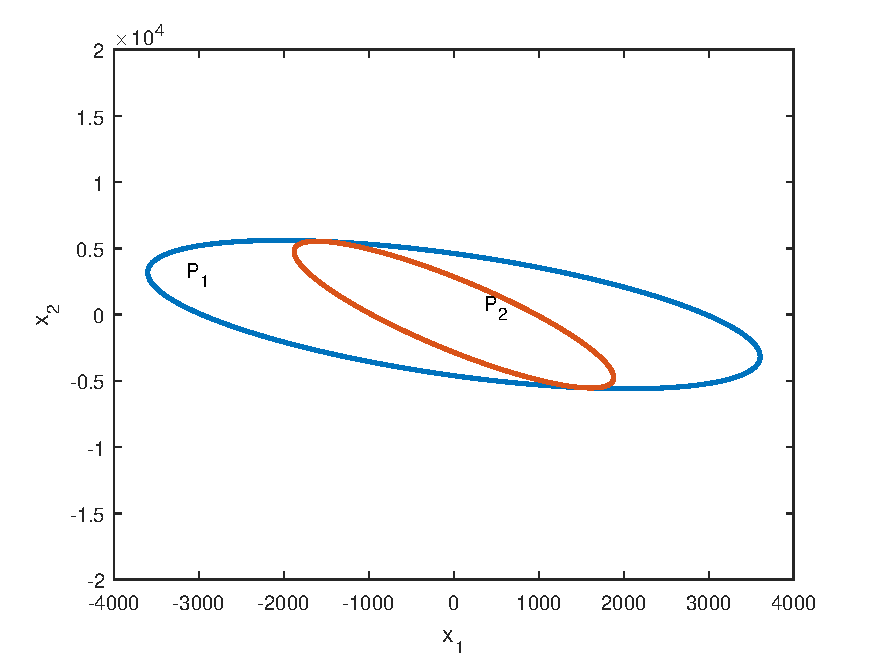
\includegraphics[width = 0.67\linewidth]{figs/switch2to1.pdf} %Linewidth ile olcekle
\caption{Example figure 1}
\label{fig:example1}
\end{figure}

\begin{figure}
\centering
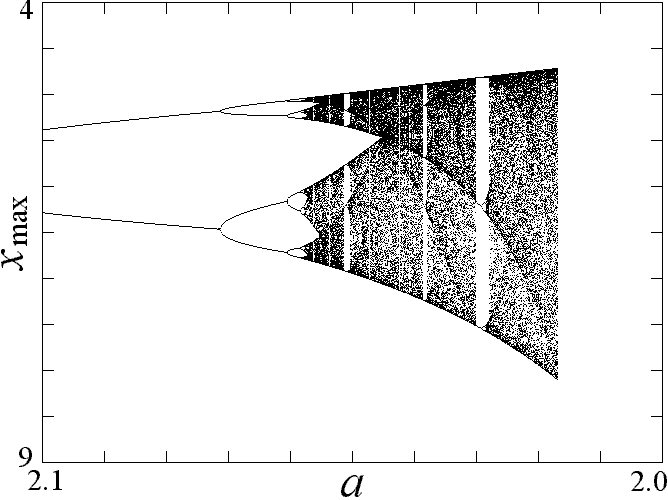
\includegraphics[width = 0.4\linewidth]{figs/bifurcation.jpg} %Linewidth ile olcekle
\caption{Example figure 2}
\label{fig:example2}
\end{figure}

\section{Third Section}

The better way of adding a figure is eps files as shown in Fig.~\ref{fig:example3}.

\begin{figure}
\centering
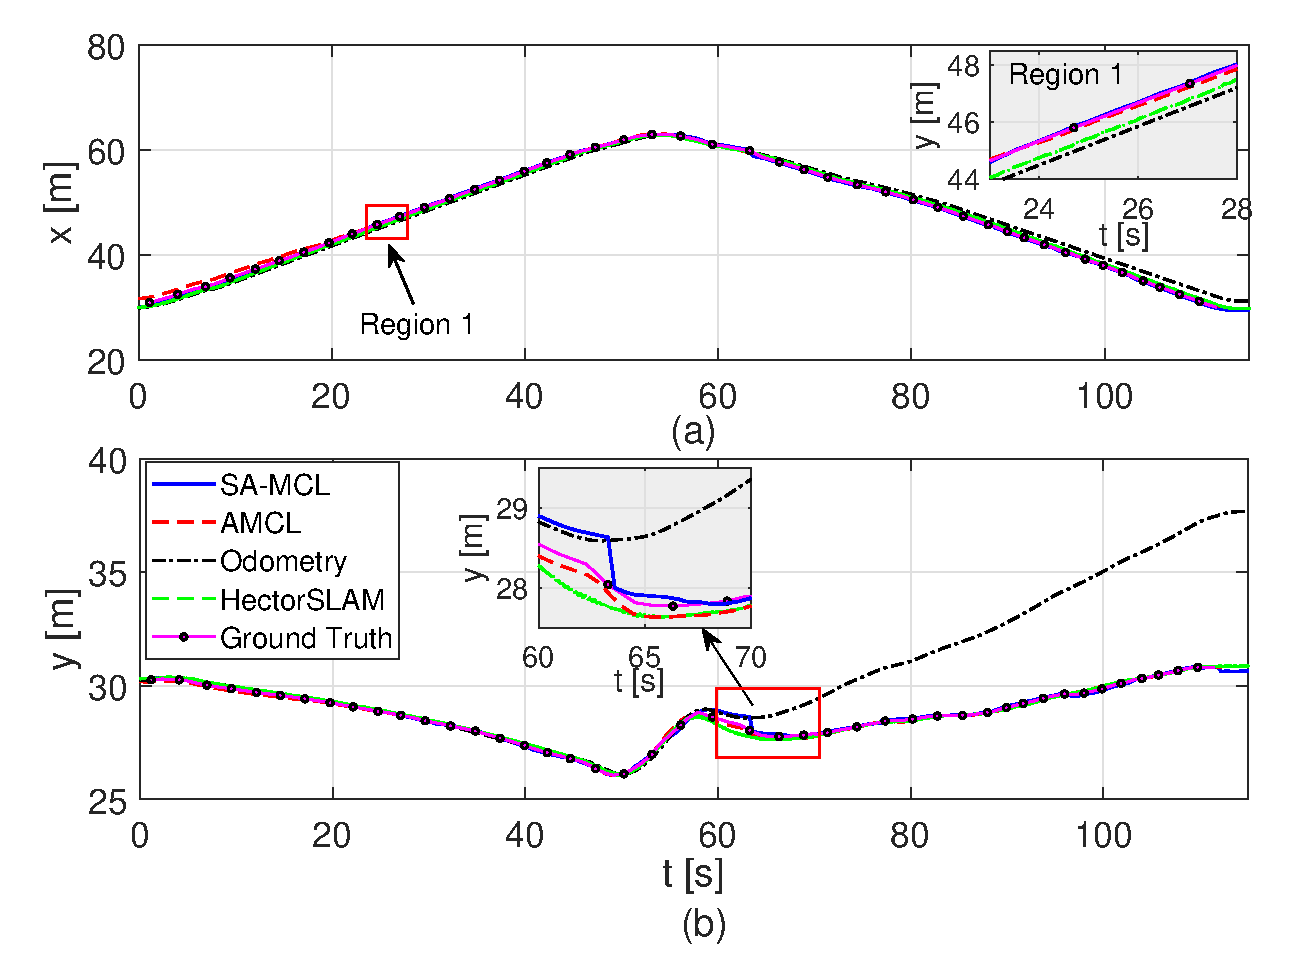
\includegraphics[width = 0.7\linewidth]{figs/deneme.eps} %Linewidth ile olcekle
\caption{Example figure 3}
\label{fig:example3}
\end{figure}

Adding text with bullets

\begin{itemize}
	\item ITU
	\item Robotics
	\item Lab
\end{itemize}

or using enumeration

\begin{enumerate}
	\item ITU
	\item Robotics
	\item Lab
\end{enumerate}


No number equation

\begin{equation*}
\label{eq:AfCorObj5} % the label is used to reference the equation
\sum_{i=1}^{\mathit{N_p}}\mathbf{x}^T \mathbb{P}_i^T C_i \mathbb{P}_i \Delta_i = \sum_{i=1}^{\mathit{N_p}}\pi_i^T C_i \mathbb{P}_i \Delta_i \Rightarrow \mathbf{x}^T\left( \sum_{i=1}^{\mathit{N_p}} \mathbb{P}_i^T C_i \mathbb{P}_i \Delta_i\right)  = \sum_{i=1}^{\mathit{N_p}}\pi_i^T C_i \mathbb{P}_i \Delta_i
\end{equation*}

Giving a reference in a sentence \cite{Rowekamper2015a}. Giving multi-reference once \cite{besl1992method,du2010affine,du2015probability,greenspan2003approximate}. \lipsum[5]

\section{Conclusions}

To put in a nut shell, in this report, we find the .... Closed form solution of the problem is shown step by step. \lipsum[4]

\bibliographystyle{IEEEtran}
\bibliography{biblio}

\end{document}
